\problemname{Coin Counter}
Given an image of a set of Swedish coins valued 1, 5 and 10 SEK, what is their sum?

The coins look like this:
\begin{figure}[h]
  \centering
  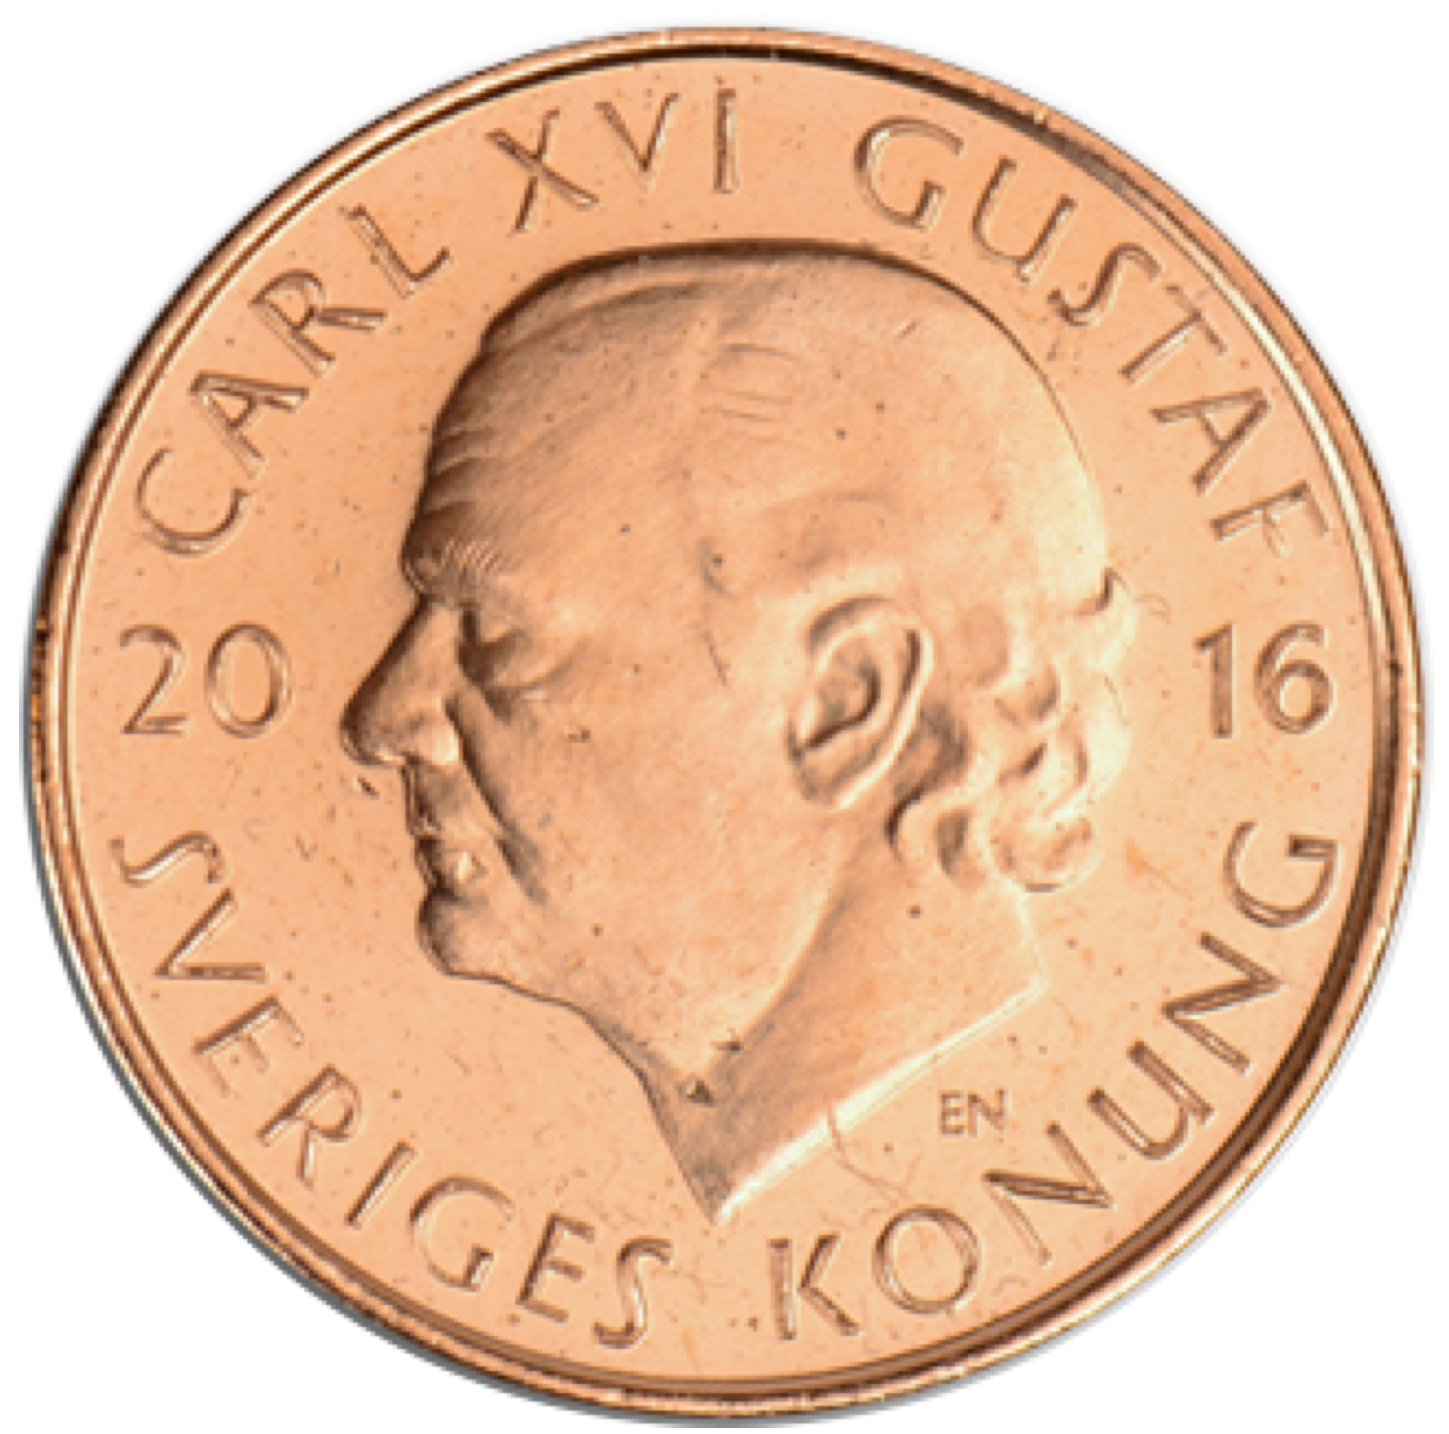
\includegraphics[width=0.2\textwidth]{1.png}
  \caption{1 SEK coin}
\end{figure}
\begin{figure}[h]
  \centering
  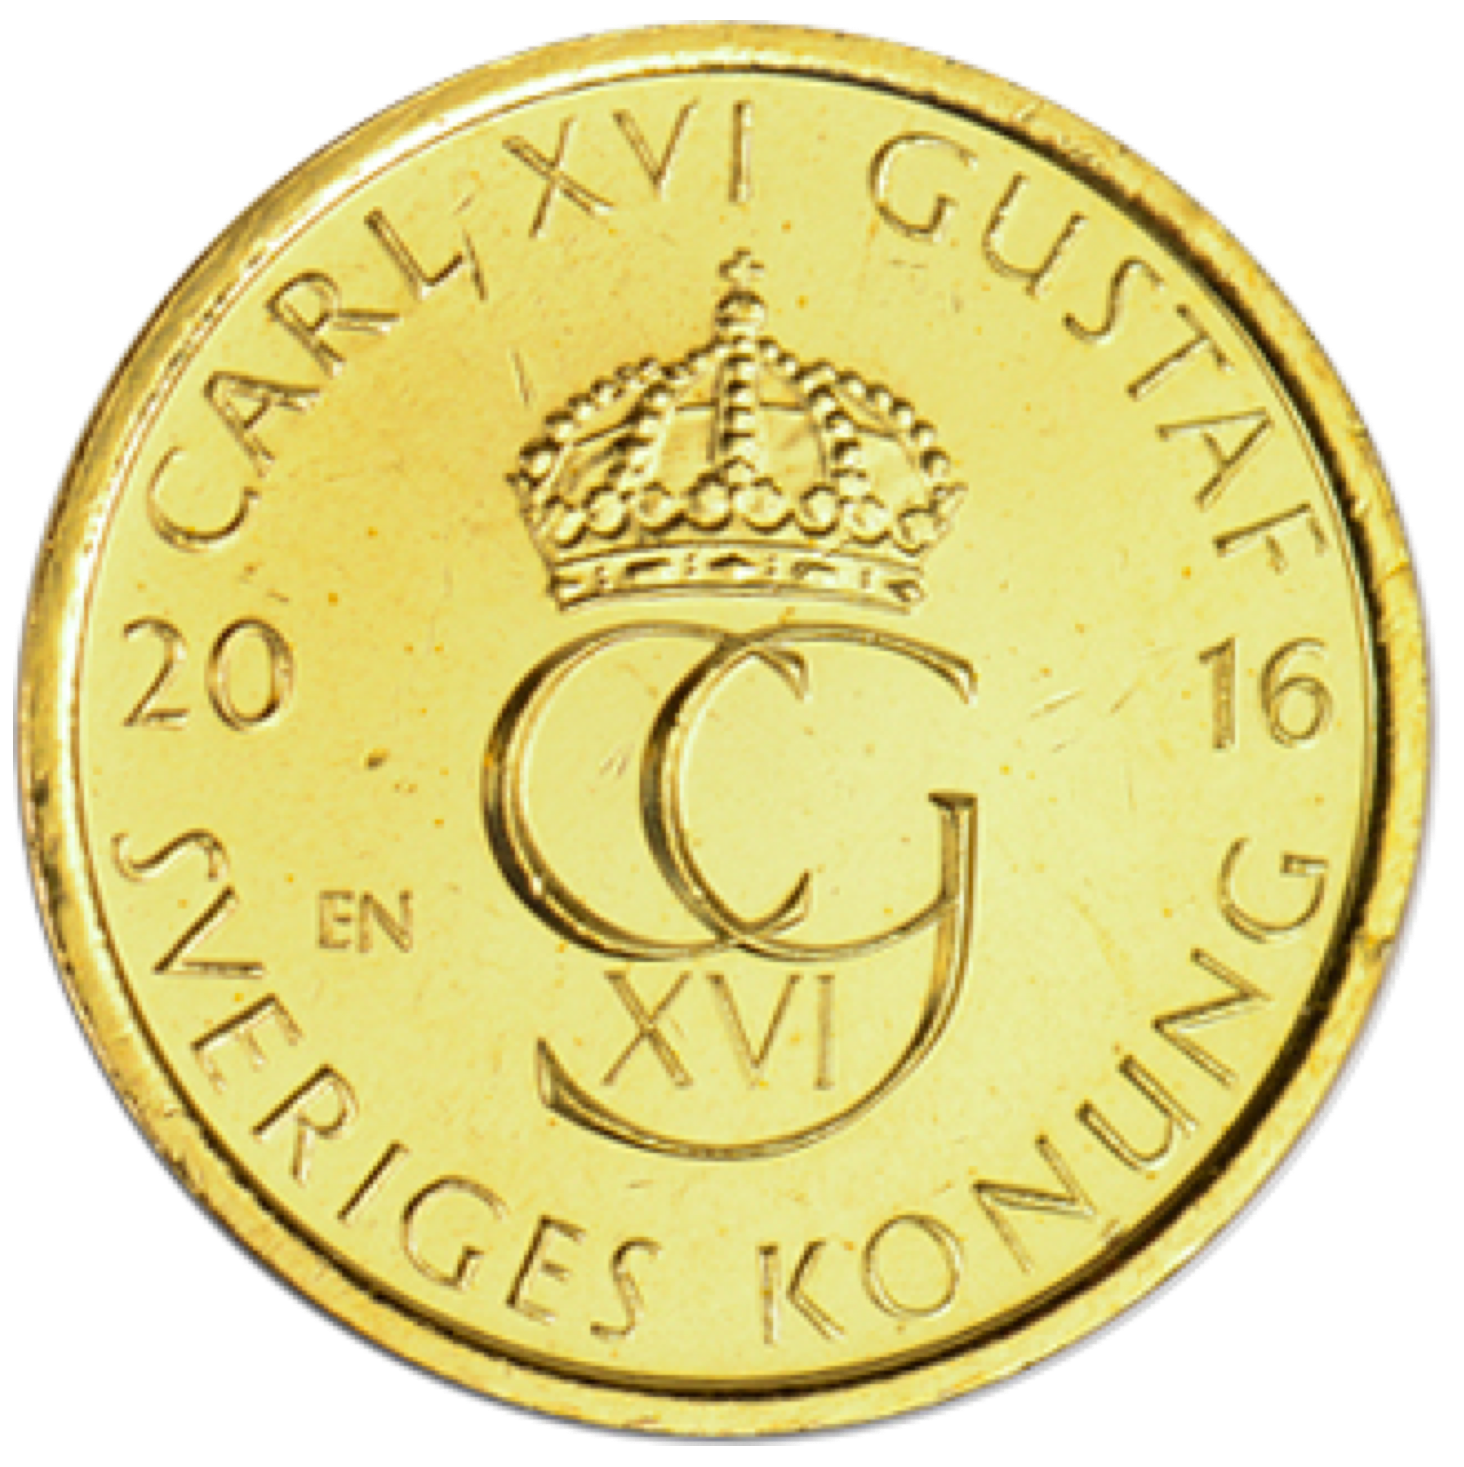
\includegraphics[width=0.2\textwidth]{5.png}
  \caption{5 SEK coin}
\end{figure}
\begin{figure}[h]
  \centering
  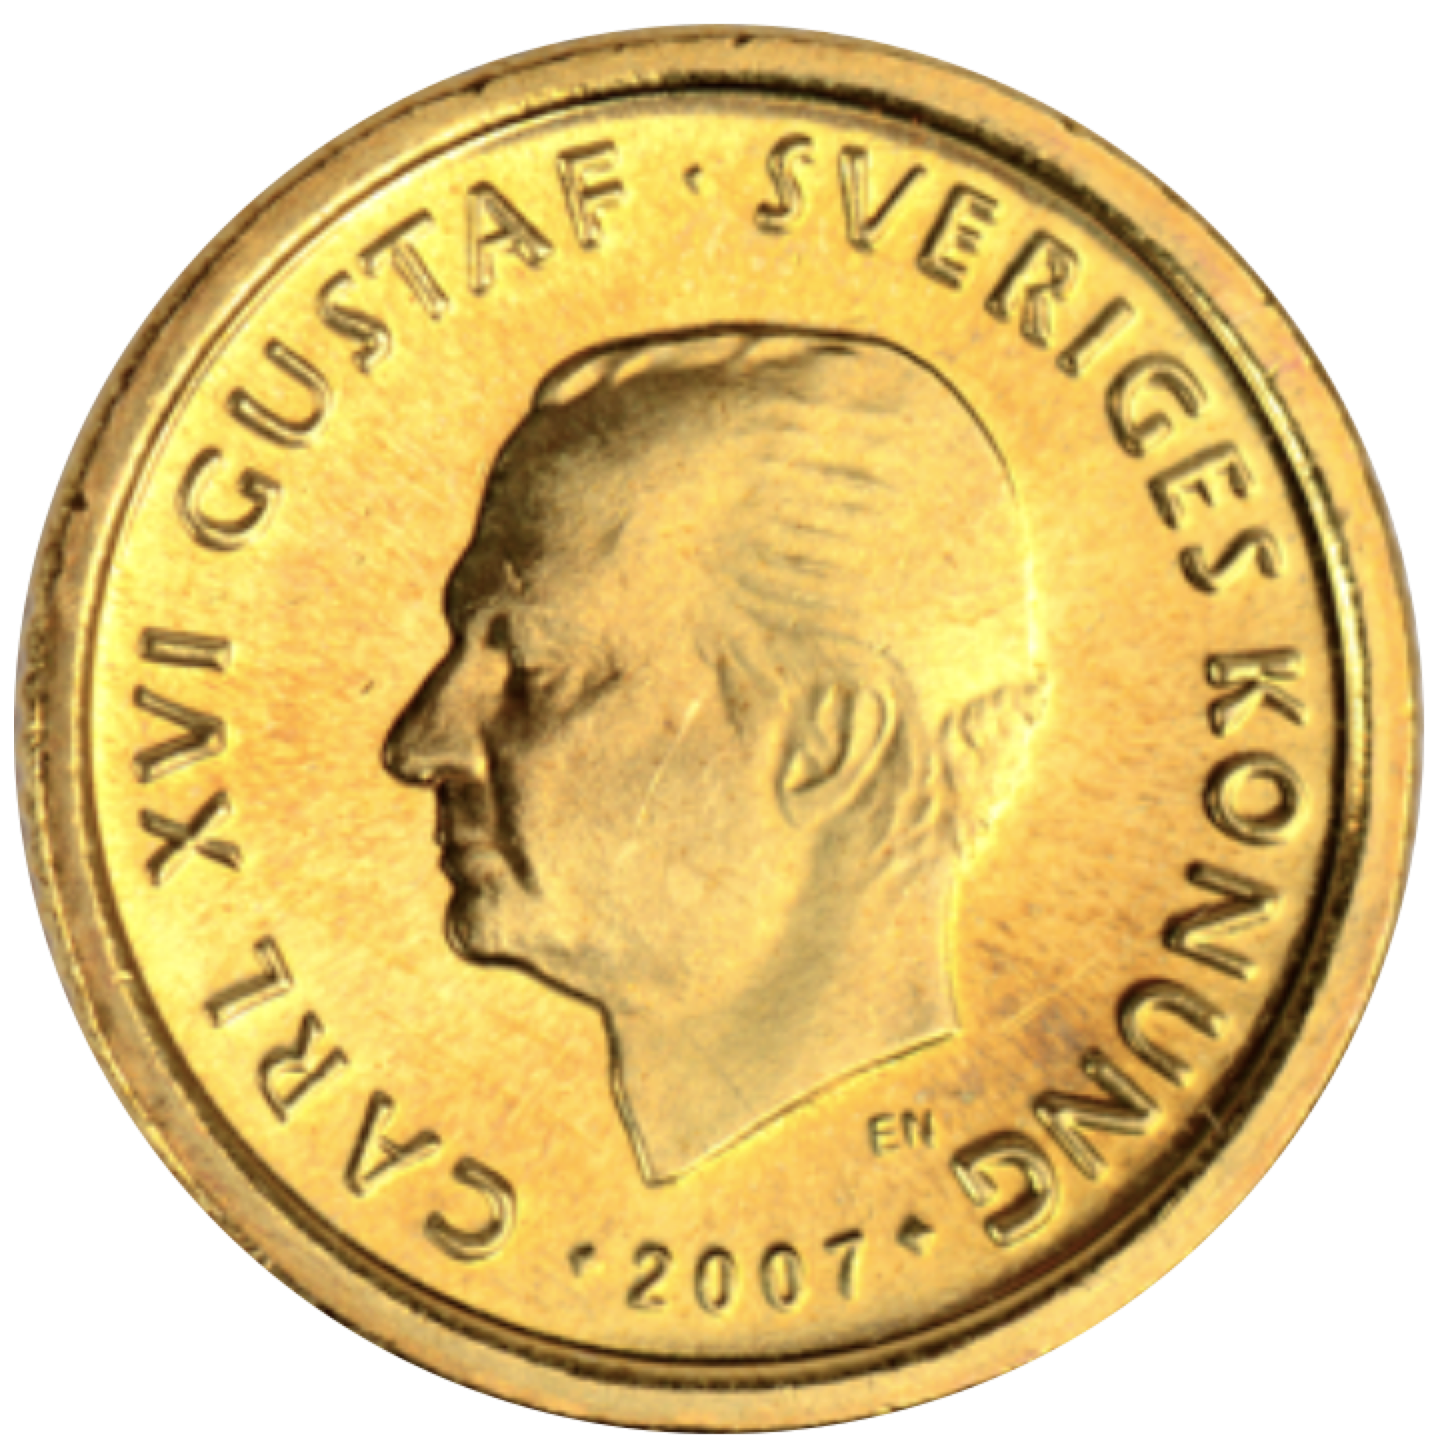
\includegraphics[width=0.2\textwidth]{10.png}
  \caption{10 SEK coin}
\end{figure}

\section*{Input}
The input is a JPEG-formatted image with dimensions $1000 \times 1000$.

No coin will be covered by other coins such that the visible parts of it is divided into two.

See the downloadable file \texttt{sampleimages.zip} in the menu to the right to download some example inputs and outputs.

Note: testing locally may be difficult on Windows, where binary files piped to stdin will have newlines converted.
For that case it is recommended to have the program read an external JPEG file, and switch to reading from stdin
when submitting to Kattis (e.g. by setting the filename to \texttt{/dev/stdin}).

\section*{Output}
Output a single number; the sum of all the coins in the input image.

\section*{Scoring}
Your solution will be tested on a set of test groups, each worth a number of points.
To get the points for a test group you need to solve all test cases in the test group.
Your final score will be the maximum score of a single submission.

\noindent
\begin{tabular}{| l | l | l |}
\hline
Group & Points & Constraints \\ \hline
1     & 20     & There are only 1 SEK coins. None of the coins are rotated or cover each other. \\ \hline
2     & 30     & There are only 1 SEK coins. None of the coins cover each other. \\ \hline
3     & 75     & There are only 1 SEK coins. \\ \hline
4     & 60     & None of the coins are rotated or cover each other. \\ \hline
5     & 90     & None of the coins cover each other. \\ \hline
6     & 225    & No further restrictions. \\ \hline
\end{tabular}
